\documentclass[fontsize=12pt,paper=a4,twoside]{scrartcl}

\newcommand{\grad}{\ensuremath{^{\circ}} }
\renewcommand{\strut}{\vrule width 0pt height5mm depth2mm}
\usepackage{multirow}
\usepackage[utf8]{inputenc}
\usepackage[final]{pdfpages}
% obere Seitenränder gestalten können
\usepackage{fancyhdr}
\usepackage{moreverb}
% Graphiken als jpg, png etc. einbinden können
\usepackage{graphicx}
\usepackage{stmaryrd}
% Floats Objekte mit [H] festsetzen
\usepackage{float}
% setzt URL's schön mit \url{http://bla.laber.com/~mypage}
\usepackage{url}
% Externe PDF's einbinden können
\usepackage{pdflscape}
% Verweise innerhalb des Dokuments schick mit " ... auf Seite ... "
% automatisch versehen. Dazu \vref{labelname} benutzen
\usepackage[ngerman]{varioref}
\usepackage[ngerman]{babel}
\usepackage{ngerman}
% Bibliographie
\usepackage{bibgerm}
% Tabellen
\usepackage{tabularx}
\usepackage{supertabular}
\usepackage[colorlinks=true, pdfstartview=FitV, linkcolor=blue,
            citecolor=blue, urlcolor=blue, hyperfigures=true,
            pdftex=true]{hyperref}
\usepackage{bookmark}

\usepackage[utf8]{inputenc}
\usepackage{colortbl}
\usepackage{listings}
\usepackage{xparse} % LaTeX 3 command
%\usepackage{ulem} % different underscores for words

\usepackage{xspace} %% Fooling LaTeX

%\uline{important}  % unterstreichen
%\uuline{urgent}    % doppelt unterstreichen
%\uwave{boat}       % unterschlängeln
%\sout{wrong}       % durchstreichen
%\xout{removed}     % ausstreichen mit

\newboolean{langversion} %Deklaration
\setboolean{langversion}{true} %Zuweisung ist 'false' für Blockkurs
\newcommand{\highlight}[1]{\textcolor{blue}{\textbf{#1}}}
\newcommand{\nurlangversion}[0]{%
\ifthenelse{\boolean{langversion}}{\highlight{Muss in SWP-2 ausgefüllt werden}}{\highlight{Entfällt in SWP-1}}}


\newcommand{\swp}[0]{\ifthenelse{\boolean{langversion}}%
{Software--Projekt 2}{Software--Projekt 1}}
\newcommand{\jahr}[0]{2014}
\newcommand{\semester}[0]{\ifthenelse{\boolean{langversion}}{WiSe}{SoSe} \jahr}

% Damit Latex nicht zu lange Zeilen produziert:
\sloppy
%Uneinheitlicher unterer Seitenrand:
%\raggedbottom

% Kein Erstzeileneinzug beim Absatzanfang
% Sieht aber nur gut aus, wenn man zwischen Absätzen viel Platz einbaut
\setlength{\parindent}{0ex}

% Abstand zwischen zwei Absätzen
\setlength{\parskip}{1ex}

% Seitenränder für Korrekturen verändern
\addtolength{\evensidemargin}{-1cm}
\addtolength{\oddsidemargin}{1cm}

\bibliographystyle{gerapali}

% Lustige Header auf den Seiten
  \pagestyle{fancy}
  \setlength{\headheight}{70.55003pt}
  \fancyhead{}
   \fancyhead[LO,RE]{\swp\\ \semester{}
  \\Projektplan}
  \fancyhead[LE,RO]{Seite \thepage\\\slshape \leftmark\\\slshape \rightmark}
  
  
  % re implements
  \lstset{literate=%
  	{Ö}{{\"O}}1
  	{Ä}{{\"A}}1
  	{Ü}{{\"U}}1
  	{ß}{{\ss}}1
  	{ü}{{\"u}}1
  	{ä}{{\"a}}1
  	{ö}{{\"o}}1
  	{°}{{$^\circ$}}1
  }

%
% Und jetzt geht das Dokument los....
%

\begin{document}

% Lustige Header nur auf dieser Seite
  \thispagestyle{fancy}
  \fancyhead[LO,RE]{ }
  \fancyhead[LE,RO]{Universität Bremen\\FB 3 -- Informatik\\
  Prof. Dr. Rainer Koschke \\TutorIn: Michaela Bunke}
  \fancyfoot[C]{}

% Start Titelseite
  \vspace{3cm}

 \begin{minipage}[H]{\textwidth}
  \begin{center}
  \bf
  \Large
  \swp{} \jahr\\
  \smallskip
  \small
  VAK 03-BA-901.02\\
  \vspace{3cm}
  \end{center}
  \end{minipage}
  \begin{minipage}[H]{\textwidth}
  \begin{center}
  \vspace{1cm}
  \bf
  {\Large Projektplan}\\
  \vspace{3ex}
  ChronoX\\% Ersetzen
  \vfill
  \end{center}
  \end{minipage}
  \vfill
  \begin{minipage}[H]{\textwidth}
  \begin{center}
  \sf
  \begin{tabular}{lrr}
  Alexander But & abut@tzi.de & 4000486\\
  Tobias Dellert & tode@tzi.de & 2936941\\
  Karsten Betjemann & mortem34@tzi.de & \color[rgb]{1,0,0} MAT\_NR\color[rgb]{0,0,0}\\
  (Tim Ellhoff & tellhof@tzi.de &  )\\
  \end{tabular}
  \\ ~
  \vspace{2cm}
  \\
  \it Abgabe: 25. Mai 2014 --- Version 1.3\\ ~
  \end{center}
  \end{minipage}

% Ende Titelseite

% Start Leerseite

\newpage

  \thispagestyle{fancy}
  \fancyhead{}
  \fancyhead[LO,RE]{\swp{}\\ \semester{} \jahr{}
  \\Projektplan}
  \fancyhead[LE,RO]{Seite \thepage\\\slshape \leftmark\\~}
  \fancyfoot{}
  \renewcommand{\headrulewidth}{0.4pt}
  \tableofcontents

\newpage

  \fancyhead[LE,RO]{Seite \thepage\\\slshape \leftmark\\\slshape \rightmark}


%%%%%%%%%%%%%%%%%%%%%%%%%%%%%%%%%%%%%%%%%%%%%%%%%%%%%%%%%%%%%%%%%%%%%%%%
\section*{Version und Änderungsgeschichte}

{\em Die aktuelle Versionsnummer des Dokumentes sollte eindeutig und gut zu
identifizieren sein, hier und optimalerweise auf dem Titelblatt.}

\begin{tabular}{ccl}
Version & Datum & Änderungen \\
\hline
1.0 & 23.05.2014 & Erste veröffentlichte Version. \\
1.1 & 24.05.2014 & Arbeitspakete, Zeitplan und Budget hinzugefügt. \\ 
1.2 & 25.05.2014 & Risikomanagement hinzugefügt. \\
1.3 & 25.05.2014 & Einleitung hinzugefügt. \\
\end{tabular}

%%%%%%%%%%%%%%%%%%%%%%%%%%%%%%%%%%%%%%%%%%%%%%%%%%%%%%%%%%%%%%%%%%%%%%%%
\setcounter{section}{-1}
\section{Über uns}

% includegraphics

%%%%%%%%%%%%%%%%%%%%%%%%%%%%%%%%%%%%%%%%%%%%%%%%%%%%%%%%%%%%%%%%%%%%%%%%
\newpage
\section{Einleitung}

\subsection{Projektübersicht}

\subsubsection{Ziele}

Im Rahmen des von unserer Gruppe angepeilten Gesamtzieles, nämlich des Bestehens vom Modul Softwareprojekt dieses Semesters, beabsichtigen wir im Bezug auf dieses Projekt sämtliche grundlegenden Kriterien zu erfüllen. Jene Kriterien beinhalten die fristgerechte Abgabe sämtlicher notwendiger Dokumente des Übungsbetriebes wie auch die Umsetzung aller Aufgaben des Miniprojektes SWP, womit unter anderem ein Projektplan, die konkrete Anforderungsspezifikation sowie die Architektur, der Testplan und der Blackbox Test der zu erarbeitenden Software eingeschlossen sind.

Der hauptsächliche Fokus unserer Arbeit wird sich dabei aufgrund des allgemeinen Aufwandes und der Bedeutung innerhalb des Moduls dem Miniprojekt zuwenden.
Hierbei beabsichtigen wir sämtliche zuvor gelisteten Mindestanforderungen für das zu entwickelnde Stundenplan-System unter Berücksichtigung aller bekanntgegebenen technischen Randbedingungen zu erfüllen und somit ein ansprechendes System zur Planung der Stundenpläne von Lehrern wie Schülern mit etwaigen Komfortfunktionen zu entwerfen.

Die oben erwähnten Mindestanforderungen definieren das zu erarbeitende System als fähig, dem Stundenplan Lehrer, Klassen und Schüler hinzufügen zu können wobei den Lehrern eine erfassbare Wochenstundenzahl zugeteilt ist.\newline
Weiterhin müssen sich die planbaren Aktivitäten in Pausen und Unterrichtsfächer aufteilen lassen können, sowie Startpunkte und Endpunkte besitzen und mehreren Klassen oder Lehrern zugleich zuteilbar sein.\newline
Darüber hinaus soll die Möglichkeit bestehen für die Lehrer und Klassen jeweils spezifische Stundenpläne anzeigen zu lassen, innerhalb derer ebenfalls die Bearbeitung und Verwaltung von Aktivitäten umsetzbar sein soll.\newline
Zuletzt soll das System zum Zweck der Problemlösung automatisch Doppelbelegungen der Lehrer oder eine im Hinblick auf die zugewiesene Wochenstundenzahl festgestellte Überbelegung anzeigen.

\subsubsection{Hauptarbeitsaktivitäten und -produkte}

Der Entwicklungsprozess eines Softwareprojektes lässt sich gemeinhin in mehrere Arbeitsaktivitäten oder auch Arbeitsphasen aufteilen, hierbei bringen die jeweiligen Arbeitsphasen ein spezifisches Arbeitsprodukt hervor, jene Arbeitsprodukte machen in unserem Fall den wesentlichen Bestandteil der Abgaben aus.\newline
Im Folgenden lässt sich anhand des klassischen Musters eine Auflistung erstellen inwiefern unser Arbeitsprozess in die Arbeitsaktivitäten aufgeteilt ist und welche Arbeitsprodukte aus ihnen resultieren.\newline

\textbf{Arbeitsaktivität - Arbeitsprodukt}

Projektplanung - Projektplan

Anforderungsanalyse - Angebotserstellung

Anforderungsspezifikation - Angebot

Entwurf - Architekturbeschreibung

Erstellung des Testplans - Testplan

Testvorgang - Tests und Testergebnisse

Implementierung - Programm

Dokumentation - Installationsanweisung und Skript

Auslieferung - Kunde erhält Produkt

\subsubsection{Haupt--Meilensteine und grober Zeitplan}

Die für dieses Projekt angesetzten Meilensteine resultieren unmittelbar aus den im Rahmen des Moduls festgelegten Abgabeterminen der einzelnen Arbeitsprodukte, abgesehen von diesen fixen Terminen, zu welchen die jeweiligen Arbeitsteile oder Gesamtarbeiten eingereicht werden müssen, werden natürlich auch vorzeitige Termine zur grundlegenden Anforderungsbesprechung oder eventueller Korrektur flexibel und auf Bedarf vor dem eigentlichen Abgabedatum eingesetzt.\newline
Im Folgenden ergibt sich für die Hauptmeilensteine deshalb ein grober Zeitplan, der genug Flexibilität ermöglicht um auf etwaige Probleme einzugehen und gleichzeitig zur organisatorischen Steuerung des Projektverlaufs verwendet werden kann.\newline

\textbf{Abgabetermin - Dokument}

18.05.2014 - Übungsblatt 1 (Zusammenfügung der Arbeitspakete vor der Abgabe)

25.05.2014 - Initialer Projektplan (Zusammenfügung der Arbeitspakete vor der Abgabe)

01.06.2014 - Übungsblatt 2 (Zusammenfügung der Arbeitspakete vor der Abgabe)

TBA - Anforderungsspezifikation (Gemeinsame Ausarbeitung und Abgabe derselben)

TBA - Architekturbeschreibung mit Schnittstellen in Java (Gemeinsame Ausarbeitung)

TBA - Testplan und JUnit-Tests (Aufteilung einzelner Tests und Fügung vor Abgabe)

Am Freitag des Blockkurs um 12 Uhr - Vollständige Abgabe (Gruppenabgabe)

\subsection{Auszuliefernde Produkte}

Die von uns auszuliefernden Produkte sind aufgrund der Art des Miniprojekt-Übungsbetriebes durch ebendiesen vorgegeben.\newline
Unsere hauptsächliche Produktleistung definiert sich also über die Erstellung von einem initialen Projektplan, der genauen Anforderungsspezifikation für die erdachte Software, der Architekturbeschreibung mit Schnittstellen in Java derselbigen, dem Testplan und der Ansammlung von über JUnit durchgeführten Tests, sowie zuletzt der vollständigen Abgabe.

\subsection{Referenzen}
% mit \nocite kann man Literatur auflisten, die im Text nicht explizit
% erwähnt ist. \nocite{*} zitiert dann das ganze .bib-File
%
% Die Bibliographie erzeugt man indem man erst
%
% pdflatex bericht.tex
% bibtex bericht
% pdflatex bericht.tex
% pdflatex bericht.tex
%
% benutzt
%\nocite{Knudsen1}
%\nocite{*}
%\bibliography{literatur}

% Das renewcommand verhindert dass für die Literatur eine section* angelegt wird.
% auftaucht
{\renewcommand\section[2]{}
	\bibliography{Referenzen}
}

Im Bezug auf etwaige Referenzen und unter Berücksichtigung der innerhalb des Projektbetriebes empfohlenen Literatur lässt sich für unser Projekt die folgende Referenzauflistung anfertigen.\newline

\emph{Ludewig, J., H. Lichter Software Engineering - Grundlagen, Menschen, Prozesse, Techniken 2. Aufl., dpunkt.verlag, Heidelberg, ISBN 978-3-89864-662-8, 2010}

\emph{R. Pressman: Software Engineering - A Practitioner's Approach. 6. Auflage, McGraw-Hill, 2004. }

\emph{I. Sommerville: Software Engineering. 8. Auflage, Addison-Wesley, 2006. }

\emph{W. Zuser, T. Grechenig, M. Köhle: Software Engineering mit UML und dem Unified Process. 2. Auflage, Pearson Studium, 2004. }

\emph{B. Brügge, A. H. Dutoit: Objektorientierte Softwaretechnik mit UML, Entwurfsmustern und Java. Pearson Studium, 2004. }

\emph{H. Störrle: UML 2 für Studenten. Pearson Studium, 2005. }

\emph{M. Dahm: Grundlagen der Mensch-Computer-Interaktion. Pearson Studium, 2005. }

\subsection{Definitionen und Akronyme}

Aufgrund der starken Nähe zur Anwendung im Alltag, welche unser Projekt auszeichnet, sind auch für das Verständnis des Projektplanes wenig Fachwissen oder Alltagskenntnisse erforderlich.\newline

\section{Projektorganisation}
\nurlangversion

\subsection{Prozessmodell}
\nurlangversion

\subsection{Organisationsstruktur}
\nurlangversion

{\em Genaue Beschreibung der Rollen, Rechte und Pflichten!}

{\em z.B. auch regelmäßiges Treffen im Chat, Einrichtung einer
	Groupware oder eines Forums, o.ä. \dots}

\subsection{Organisationsgrenzen und --schnittstellen}
\nurlangversion

{\em Hierher gehören auch evtl. Kontaktpersonen für Fremdbibliotheken u.ä.}

\subsection{Verantwortlichkeiten}
\nurlangversion

\section{Managementprozess}

\subsection{Managementprozess und --prioritäten}

\subsection{Annahmen, Abhängigkeiten und Einschränkungen}

\subsection{Risikomanagement}\label{riskmanagement}

{\em Wenn Ihr Euch entschieden habt, bestimmte vorbeugende Maßnahmen 
     durchzuführen, solltet Ihr dies deutlich kennzeichnen. Hoffentlich
     haben diese Maßnahmen dann einen Einfluss auf Eintrittswahrscheinlichkeit oder Schadenshöhe (zum Beispiel
     ist die Eintrittswahrscheinlichkeit von komplettem Datenverlust durch regelmäßige Backups deutlich 
     geringer). Daher solltet Ihr für diese Fälle dann die verringerten Werte für Eintrittswahrscheinlichkeit, 
     Schadenshöhe und Risikopotential zusätzlich angeben. }

{\em Wie werden neue Risiken erkannt/erfasst? Wer ist für was
  zuständig? Wie ist der Informationsfluss? \ldots 

Dieser Teil ist ein
  wichtiger Schwerpunkt des Projektplans und sollte daher ausführlich
  behandelt werden.}

Um eine schnellere Erfassung der Risiken zu bekommen, eignen sich immer visuelle Darstellungen. Wir verwenden dafür eine Matrix/Tabelle, bei der man die Risikostufen schnell erkennen kann.\\

\begin{figure}[H]
	\centering
	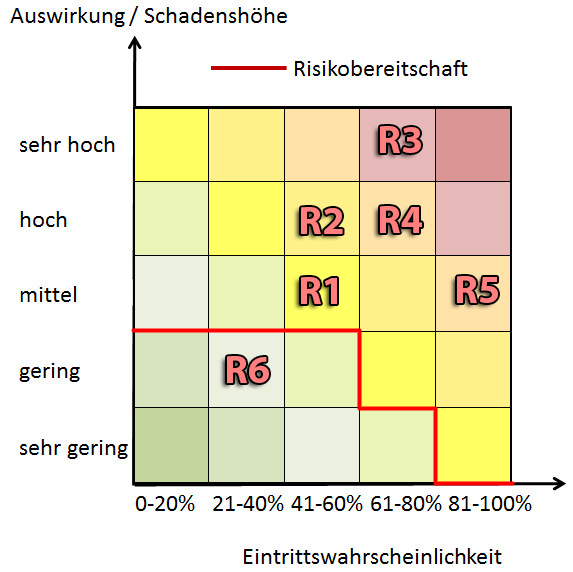
\includegraphics[width=0.75\textwidth]{src/risikomatrix_before.png}
	\caption{Risikomatrix vor Maßnahmenergreifung}
	\label{fig:matrixtable_before}
\end{figure}

\subsubsection{(Mögliche) Risiken}


\begin{tabbing}
	\hspace*{5em}\= \kill
	\textbf{R1:}\> Ein Gruppenmitglied kann nicht progra-\\
				\> mmieren.\\[0.5em]
	\textbf{R2:}\> Am Tag des Blockkurses sind mindst. 2\\
				\> Gruppenmitglieder nicht anwesend/ver-\\
				\> hindert.\\[0.5em]
	\textbf{R3:}\> Konflikte bahnen sich an, die den erfolg-\\
				\> reichen Abschluss des Projektes gefährden.\\[0.5em]
	\textbf{R4:}\> (Interne) (Gruppen-)Kommunikationen\\ 
				\> kommen nicht (erfolgreich) zustande.\\[0.5em]
	\textbf{R5:}\> Festgelegte Auflagen werden (oft) nicht\\
				\> eingehalten.\\[0.5em]
	\textbf{R6:}\> Der/Die BetreuerIn/TutorIn/AufpasserIn\\
				\> fällt für längere Zeit aus.\\[0.5em]
\end{tabbing} 

\textbf{R1:} Eine Erklärung ist wohl nicht von Nöten. Wenn man sich die Ausgangssituation ausschaut, kann entweder einer/eine programmieren oder nicht. Es wären ca. 50\%. Der Schaden wären mittel bis hoch, da man programmieren muss, um den Stundenplan erstellen zu können. Noch kann man nicht durch pure Gedankenkraft, materiale Gegenstände erzeugen. Sehr schlimm wird es, wenn das Risiko kurz vor der Implementierung entdeckt wird.\\

Das Auslösen dieses Risikos kann (gänzlich) vermieden werden, wenn man zuvor Eignungstests bzw. Programmiertests durchführt. Noch kann man der Person helfen. Sobald das Wintersemester anfängt, wird dieses Risiko zu 100\% eintreten, wenn es wirklich eine Person mit diesem Defizit gibt. Jede Hilfe wäre dann vergebens.\\ 

\textbf{R2:} Sowas kann immer vorkommen, da plötzlich einer krank wird, die Bahn mal wieder im "`Eiltempo"' die Passagieren verärgert oder ganz schlicht einer verschläft.
Lustlosigkeit, da es in der vorlesungsfreien Zeit stattfindet, soll wohl auch schon mal vorgekommen sein.\\

Es wäre ein Desaster auf hohem Niveau, da spontan Überstunden zu praktizieren, nicht mehr einplanbar wäre. Dieses Risiko einzuschätzen, wie wahrscheinlich es eintrifft, ist de facto kaum möglich. Die Indikatoren sind nämlich (fast) nicht vom Menschen beeinflussbar.\\
Das Miniprojekt fertig zu stellen, würde in die weite Ferne rücken.\\
Präventionspläne kann man nicht realisieren. Da hilft wohl nur, einen (oder mehrere) Alternativpläne vorzubereiten und wenn das Risiko auftreten sollte, wenigstens das Nötigste zu implementieren. Man würde den Schaden begrenzen.\\ 

\textbf{R3:} Ein oft unterschätztest Risiko. Konflikte werden bei jeder Gruppe auftreten. Das ist unvermeidbar. Glücklicherweise sind diese Konflikte nicht allzu groß und lösen sich schnell wieder auf. Das gilt jedoch nicht für alle. Die meisten ernstzunehmenden Konflikte entwickeln sich aus kleineren [Konflikten], die wie zuvor genannt, unterschätzt werden. Dies kann nicht nur die Zusammenarbeit dauerhaft schädigen, sondern auch das Projekt zum Sterben verdammen. Unserer Einschätzung nach, gehört es zu den Gefährlichsten Risiken, die wir identifizieren konnten (siehe Abb.~\ref{fig:matrixtable_before}).\\

So gefährlich es ist, so leicht lässt es sich lösen. Man muss das Problem an der Wurzel packen und es erst gar nicht entfalten lassen. Schon Gruppenmeetings, Gespräche mit einer neutralen Person (TutorIn, ProfessorIn) wirken Wunder, auch wenn man es nicht glauben kann.\\
So könnte man den Schaden bis aufs Minimum drücken und die Wahrscheinlichkeit etwas senken.\\
Ausnahmen bestätigen die Regeln. Manche Konflikte sind - mit der derzeitigen Konstellation - nicht lösbar. Da hilft nur eine Gruppentrennung, damit beide Seiten den Kollateralschaden möglichst gering halten können.\\

\textbf{R4:} Dieses Risiko soll 2 Fälle beinhalten.\\ Den ersten Fall mussten wir schon recht früh selbst erleben. 2 Gruppenmitglieder haben auf verschiedensten Kommunikationswegen einfach zu spät bis gar nicht geantwortet. Um ein Bildnis machen zu können: 1-3 Wochen dauerte es, bis auf Fragen und anderen (organisatorischen) Aufgaben, erwidert wurde. Nicht nur das es unhöflich ist - zumindest in Europa, es bringt die ganze Planung (Zeitmanagement und Taskmanagement) durcheinander. Zwar ist es üblich, dass Pläne nicht eingehalten werden, jedoch ist keine allzu hohe Varianz vorhanden. (Es müsste sich auf 5\% belaufen, jedoch habe ich keine Quelle parat und somit sollte diese Aussagen nur als These angenommen werden.)\\
Der zweite Fall ist die Misskommunikation. Man hat sich verhört oder hat es sich so eingebildet, als hätte man es so gesagt.\\
Das man mal etwas (akustisch) nicht mitbekommt, bedeutet noch nicht das eindeutige Aus. Es kann jedoch den kritischen Pfaden "`verlängern"'. D.h., Aufgaben, Prozesse, die eine hohe Abhängigkeit besitzen, müssen verschoben werden. Autarke Prozesse zu erstellen, ist nicht immer möglich bzw. Vorteilhaft.\\
Eine mögliche Vorbeugung: Alles Wichtige wird nochmal als expliziertes wissen manifestiert (z.B. auf Papier, in einer E-Mail, im Forum, ...). Die Schadenshöhe würde auf dem gleichen Level bleiben. Die Eintrittswahrscheinlichkeit würde sinken, da man eventuell die Informationen immer wieder sich durchlesen könnte. Verbales wird im primären Gedächtnis gespeichert und rund 80\% davon sind innerhalb des nächsten halben Tages "`verschwunden"'.\\ 


\textbf{R5:} Das sowas eintreten kann, ist hoch, da wir neben SWP auch noch andere akademische Tätigkeiten vollführen und manche noch Arbeiten gehen. Der Schaden kann in alle möglichen Stufen auftreten. Wir haben uns für den Durchschnitt entschieden und das Mittelmaß gewählt (siehe Abb.~\ref{fig:matrixtable_before}).
Zur Vorbeugung der Schadenshöhe, haben wir einen Auflagenkatalog erstellt, der bis Juli 2014 die finale Phase erreichen wird. Damit es keine Missverständnisse geben soll, muss sich jedes Gruppenmitglied diesen Katalog durchlesen und auch zustimmen (Unterschrift). Da wir es Gruppenintern belassen wollen, wird hier nur ein kleiner Ausschnitt gezeigt:\\

\small Jeder hat ein Kontigent von \color{red}{11 Punkten}\color{black}\\[0.7em]
\small Wer diese Punktzahl erreicht bzw. überschreitet, wird aus der Gruppe \color{red}{ausgeschlossen}\color{black}!\\[0.7em]

\small Person meldet sich erst \color{blue}{nach 2 Tagen ohne Begründung}\color{black}\\
\small $->$ \color{red}{3,5 }\color{black} Punkte\\

\small Person gibt widerholt nicht ab\\
\small $->$ \color{red}{5,5 }\color{black} Punkte\\

\small Person kommt innerhalb \color{blue}{eines Monats }\color{black} insgesamt \color{blue}{30min }\color{black} zu spät\\
\small $->$ \color{red}{2,0 }\color{black} Punkte\\

\small Zuvor zugesagte Aufgaben werden nicht erledigt (und die anderen nicht darüber informiert)\\
\small $->$ \color{red}{1,5 }\color{black} Punkte\\

\small Person macht nichts/stachelt bewusst Konflikte an\\
\small $->$ \color{red}{8,0 }\color{black} Punkte\\

\small Person will unbedingt  die Gruppe durchfallen lassen\\
\small $->$ \color{red}{11,0 }\color{black} Punkte\\

\small Es wurde wiederholt nicht nach Auflagen gehalten (Schreibtool, Dokumentsprache, falsches CVS, ...)\\
\small $->$ \color{red}{jeweils 1,0 }\color{black} Punkte\\

\small Interne Deadlines wurden nicht eingehalten - und nicht rechtzeitig informiert\\
\small $->$ \color{red}{0,5 - 2,5 (je nach Häufigkeit) }\color{black} Punkte\\

\small \color{gray} Person erledigt mehr Aufgaben als besprochen wurde - bei einer konstant hohen Qualität\color{black}\\
\small $->$ \color{green}{-3,5 }\color{black} Punkte\\

\small \color{gray} Person investiert mehr Zeit (freiwillig) z.B. Überstunden (mit einer Oberschranke)\color{black}\\
\small $->$ \color{green}{-1,0 - -5,0 }\color{black} Punkte\\

\small \color{blue} Alle 2 Wochen fällt der Kontostand um 7 Punkte!\color{black}\\

\textit{Ein Programm übernimmt diese Aufgaben.}\\

\textbf{R6:} Bei diesem Risiko sind uns die Hände gebunden. Zwar ist der Schaden und der Eintritt gering, jedoch können wir es nicht weiter kompensieren.\\

Es ist aber auch das Risiko, bei dem wir die Schadenshöhe von Beginn an akzeptieren.\\


\begin{figure}[H]
	\centering
	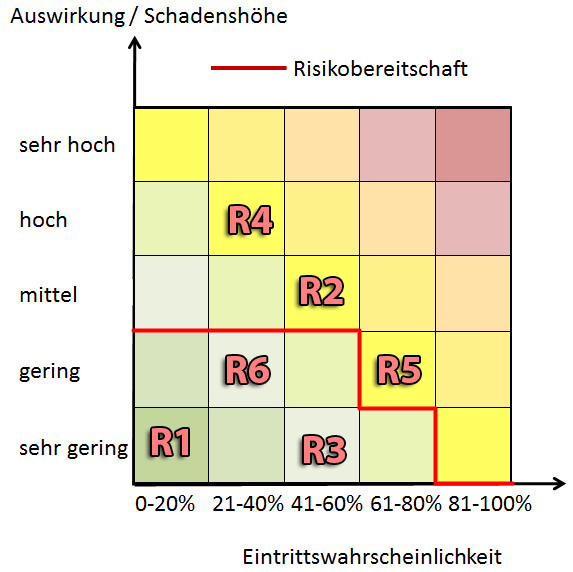
\includegraphics[width=0.75\textwidth]{src/risikomatrix_after.png}
	\caption{Risikomatrix nach Maßnahmenergreifung}
	\label{fig:matrixtable_after}
\end{figure}


\subsection{Projektüberwachung}\label{sec:controlling}
{\em Wie wird der Projektstatus verfolgt? Wie stellt Ihr sicher, dass
  der Phasenleiter jederzeit über den Stand der Entwicklung informiert
  ist? Wie werden Probleme bzw. Verzögerungen frühzeitig erkannt und
  angegangen?}\\

Wir treffen uns mindestens einmal die Woche und geben den Status quo wider. Bei Anomalien wird sofort benachrichtigt, gewarnt und gehandelt, damit man eventuell Krisensitzungen abhalten kann. Notfalls wird eine Skype-Videokonferenz abgehalten, wenn es nicht anders geht.\\
Im Blockkurs werden wir uns an die Meilensteine (grob) richten. Alle 2h wird der derzeitige Stand (kurz) geschildert. Ebenso Vorschläge als auch Probleme bzw. Prognosen zu zukünftigen Problemen, da 12 Augen mehr erblicken können, als nur ein Einzelner.\\ 

\subsection{Mitarbeiter}
{\em Kompetenzen der und Anforderungen an die Mitarbeiter.}

Die Anzahl der Anforderungen ist - in diesem Fall - recht überschaubar, jedoch im Detail komplex.\\
Ein Minimum an Java-Kenntnissen reicht nur in der Theorie aus. Objektorientierung, Fehleranalyse und Kreation von effizienten Algorithmen, sollte man auch vorweisen können, da kein Kunde gerne 10min wartet, bis eine große Datenbank geladen hat und die Werte erst dann auf dem Bildschirm darstellt.\\
Natürlich ist es nicht der Standard. Es wird (verständlicherweise) immer Gruppenmitglieder geben, die eine Sache nicht vorweisen können.\\
Um dieser Lage Herr zu werden, ist eine optimale Aufgabenaufteilung erforderlich. Dazu später mehr [\ref{sec:arbeitspaket_zeitplan_budegt}]\\

Beobachtung und Analyse wären auch sehr empfehlenswert, wenn man später die Anforderungsspezifikation erstellen muss und in der Ist-/Soll-Phase, Personas-Phase, ... sich befindet. Da es keine richtigen Anforderungen sind und langsam am Thema vorbei geschrieben wird, wird dieser Aspekt offen in dem Raum gestellt.\\ 

%%%%%%%%%%%%%%%%%%%%%%%%%%%%%%%%%%%%%%%%%%%%%%%%%%%%%%%%%%%%%%%%%%%%%%%%

\section{Technische Prozesse}
\nurlangversion
\subsection{Methoden, Werkzeuge und Techniken}
\nurlangversion
\subsubsection{Entwicklungsplattform}

\subsubsection{Entwicklungsmethode}
{\em Ist der Einsatz spezieller Methoden vorgesehen?}

\subsubsection{Programmiersprache und Bibliotheken}

\subsection{Dokumentationsplan}
\nurlangversion

\subsubsection{Codingstyle}

\subsubsection{Kommentarsprache}

\subsubsection{JavaDoc}

\subsubsection{Begleitende Dokumentation}

\subsection{Unterstützende Projektfunktionen}
\nurlangversion
{\em Wie wird Euer Konfigurationsmanagement funktionieren? Wer ist verantwortlich? Benötigt Ihr dazu Ressourcen oder Zeit? Plant Ihr Datensicherung?}

{\em Gibt es Maßnahmen zur Qualitätssicherung? Wer ist zuständig?
  Wieviel Zeit ist dafür vorgesehen?}


%%%%%%%%%%%%%%%%%%%%%%%%%%%%%%%%%%%%%%%%%%%%%%%%%%%%%%%%%%%%%%%%%%%%%%%%

\section{Arbeitspakete, Zeitplan und Budget} 
\label{sec:arbeitspaket_zeitplan_budegt}

{\em Dieser Teil ist ein zweiter Schwerpunkt des Projektplans. Hier sollt Ihr die nächste Phase detailliert planen (siehe Arbeitspakete). Die weiteren Phasen sollen ebenfalls wenigstens grob geplant werden. Ein Gantt-Diagramm ist zwingend! 
	
	Ihr sollt den Plan in der kommenden Phase auch tatsächlich benutzen -- und so
	Erfahrungen sammeln, was evtl. bei der Planung unberücksichtigt
	blieb. Bei der nächsten Zeitplanung (für die nächste Phase) bekommt
	Ihr dann evtl.\ eine noch bessere Planung hin.}

\subsection{Arbeitspakete}\label{aps}
\begin{figure}
	\includegraphics[angle = 90, scale=0.5]{as.png}
	\caption{Anforderungsspezifikation im Gantt-Diagramm}
	\label{Gantt-AS}
\end{figure}

{\em Besonderen Wert legen wir auf die Granularität der APs. Diese
	sollten von 1-2 Personen in max. einer Woche Zeitdauer (kalendarisch, nicht
	Aufwand) bearbeitbar sein. Die Beschreibungen sollten so genau sein,
	dass der Bearbeiter damit genau weiß, was zu tun ist.}




\begin{tabular}{|p{5.3cm}|p{9.7cm}|}\hline
	\textbf{Arbeitspaket Nr.:} 1.0 & \textbf{Bezeichnung:} Anforderungsspezifikation\\ \hline \hline
	\textbf{Beginn} & 01.06.14\\ \hline
	\textbf{Ende} & 06.07.14\\ \hline
	\textbf{Zuständig} & Alle\\ \hline
	\textbf{Ressourcen} & \begin{itemize}
		\item Alle
	\end{itemize}    \\ \hline
	\textbf{Abhängigkeit} &\\ \hline
	\textbf{Aufwand} & \\ \hline
	\textbf{Dauer} & \\ \hline
	\multicolumn{2}{|p{15cm}|}{\textbf{Beschreibung:}\newline   }\\ \hline
	\multicolumn{2}{|p{15cm}|}{\textbf{Mindestkriterien:}\newline }\\ \hline
\end{tabular}

\begin{verbatim} 
\end{verbatim}

\begin{tabular}{|p{5.3cm}|p{9.7cm}|}\hline
	\textbf{Arbeitspaket Nr.:} 1.1 & \textbf{Bezeichnung:} Gruppentreffen\\ \hline \hline
	\textbf{Beginn} & 01.06.14\\ \hline
	\textbf{Ende} &  01.07.14\\ \hline
	\textbf{Zuständig} Alle \\ \hline
	\textbf{Ressourcen} & \begin{itemize}
		\item 
		\item blaa
	\end{itemize}    \\ \hline
	\textbf{Abhängigkeit} &\\ \hline
	\textbf{Aufwand} & 8h\\ \hline
	\textbf{Dauer} & ?\\ \hline
	\multicolumn{2}{|p{15cm}|}{\textbf{Beschreibung:}\newline  Um die Qualität der einzelnen Bearbeitungen sicherzustellen und eine Möglichkeit für Fragen und Besprechungen zu bieten, werden wir uns als Gruppe mindestens einmal in der Woche gemeinsam treffen. }\\ \hline
	\multicolumn{2}{|p{15cm}|}{\textbf{Mindestkriterien:}\newline Jeder Arbeitsvorgang kann bei Bedarf ausreichend für die weitere Bearbeitung besprochen werden. }\\ \hline
\end{tabular}

\begin{verbatim} 
\end{verbatim}

\begin{tabular}{|p{5.3cm}|p{9.7cm}|}\hline
	\textbf{Arbeitspaket Nr.:} 1.2 & \textbf{Bezeichnung:} GUI-Prototyp\\ \hline \hline
	\textbf{Beginn} & 02.06.14\\ \hline
	\textbf{Ende} & 16.06.14\\ \hline
	\textbf{Zuständig} & Tobias Dellert\\ \hline
	\textbf{Ressourcen} & \begin{itemize}
		\item Alexander But
	\end{itemize}    \\ \hline
	\textbf{Abhängigkeit} &\\ \hline
	\textbf{Aufwand} & 16h\\ \hline
	\textbf{Dauer} & \\ \hline
	\multicolumn{2}{|p{15cm}|}{\textbf{Beschreibung:} Der hier erstellte Prototyp soll die Beschaffenheit der späteren Benutzeroberfläche darstellen. \newline   }\\ \hline
	\multicolumn{2}{|p{15cm}|}{\textbf{Mindestkriterien:} Der Kunde ist mit dem Prototypen einverstanden.\newline }\\ \hline
\end{tabular}

\begin{verbatim} 
\end{verbatim}

\begin{tabular}{|p{5.3cm}|p{9.7cm}|}\hline
	\textbf{Arbeitspaket Nr.:} 1.2.1 & \textbf{Bezeichnung:} Story-Board\\ \hline \hline
	\textbf{Beginn} & 02.06.14\\ \hline
	\textbf{Ende} & 02.06.14\\ \hline
	\textbf{Zuständig} & Tobias Dellert\\ \hline
	\textbf{Ressourcen} & \begin{itemize}
		\item Tobias Dellert
	\end{itemize}    \\ \hline
	\textbf{Abhängigkeit} & -\\ \hline
	\textbf{Aufwand} & 1h\\ \hline
	\textbf{Dauer} & 1 Tag\\ \hline
	\multicolumn{2}{|p{15cm}|}{\textbf{Beschreibung:}\newline  Das Story-Board beschreibt die erforderlichen Darstellungen, um die möglichen Vorgänge abzudecken }\\ \hline
	\multicolumn{2}{|p{15cm}|}{\textbf{Mindestkriterien:}\newline Alle mögliche Vorgänge sind abgedeckt. }\\ \hline
\end{tabular}

\begin{verbatim} 
\end{verbatim}

\begin{tabular}{|p{5.3cm}|p{9.7cm}|}\hline
	\textbf{Arbeitspaket Nr.:} 1.2.2 & \textbf{Bezeichnung:} Design\\ \hline \hline
	\textbf{Beginn} & 03.02.14\\ \hline
	\textbf{Ende} & 03.02.14\\ \hline
	\textbf{Zuständig} & Alexander But\\ \hline
	\textbf{Ressourcen} & \begin{itemize}
		\item Alexander But
	\end{itemize}    \\ \hline
	\textbf{Abhängigkeit} & -\\ \hline
	\textbf{Aufwand} & 4h\\ \hline
	\textbf{Dauer} & 1 Tag\\ \hline
	\multicolumn{2}{|p{15cm}|}{\textbf{Beschreibung:}Hier werden die einzelnen Bestandteile des Prototypen gestaltet.\newline   }\\ \hline
	\multicolumn{2}{|p{15cm}|}{\textbf{Mindestkriterien:} Das Design soll den Wünschen des Kunden bestmöglich entsprechen\newline }\\ \hline
	
\end{tabular}
\begin{verbatim} 

\end{verbatim}
\begin{tabular}{|p{5.3cm}|p{9.7cm}|}\hline
	\textbf{Arbeitspaket Nr.:} 1.2.3 & \textbf{Bezeichnung:} Entwicklungsphase I \\ \hline \hline
	\textbf{Beginn} & 04.06.14\\ \hline
	\textbf{Ende} & 06.06.14\\ \hline
	\textbf{Zuständig} & Tobias Dellert \\ \hline
	\textbf{Ressourcen} & \begin{itemize}
		\item Tobias Dellert
		\item Alexander But
	\end{itemize}    \\ \hline
	\textbf{Abhängigkeit} & Story-Board, Design\\ \hline
	\textbf{Aufwand} & 16h\\ \hline
	\textbf{Dauer} & 3 Tage\\ \hline
	\multicolumn{2}{|p{15cm}|}{\textbf{Beschreibung:}\newline Das Konzept von Stroy-Board und Design wird umgesetzt. Die Ergebnisse der ersten Entwicklungsphase werden dem Kunden vorgestellt.  }\\ \hline
	\multicolumn{2}{|p{15cm}|}{\textbf{Mindestkriterien:}\newline Die Entwicklungsphase ist ein Ergebnis aus dem Story-Board und dem Design, welche auf dem Verständnis der Wünsche des Kunden basieren.}\\ \hline
	
\end{tabular}
\begin{verbatim} 

\end{verbatim}
\begin{tabular}{|p{5.3cm}|p{9.7cm}|}\hline
	\textbf{Arbeitspaket Nr.:} 1.2.4 & \textbf{Bezeichnung:} GUI-Prototyp-Vorstellung\\ \hline \hline
	\textbf{Beginn} & 11.06.14\\ \hline
	\textbf{Ende} &11.06.14\\ \hline
	\textbf{Zuständig} & Tobias Dellert\\ \hline
	\textbf{Ressourcen} & \begin{itemize}
		\item Tobias Dellert
		\item Alexander But
	\end{itemize}    \\ \hline
	\textbf{Abhängigkeit} & Entwicklungsphase I\\ \hline
	\textbf{Aufwand} & 6h\\ \hline
	\textbf{Dauer} & 1 Tag\\ \hline
	\multicolumn{2}{|p{15cm}|}{\textbf{Beschreibung:}\newline  Das Ergebnis der ersten Entwicklungsphase wird dem Kunden vorgestellt. Es wird bestmöglich versucht die Meinung des Kunden dazu und eventuelle Verbesserungswünsche zu verstehen. }\\ \hline
	\multicolumn{2}{|p{15cm}|}{\textbf{Mindestkriterien:}\newline Die Meinung des Kunden wurde erfasst und das weitere Vorgehen beim GUI-Prototypen ist klar.}\\ \hline
	
\end{tabular}
\begin{verbatim} 

\end{verbatim}
\begin{tabular}{|p{5.3cm}|p{9.7cm}|}\hline
	\textbf{Arbeitspaket Nr.:} 1.2.5 & \textbf{Bezeichnung:} Entwicklungsphase II\\ \hline \hline
	\textbf{Beginn} & 12.06.14\\ \hline
	\textbf{Ende} & 16.06.14\\ \hline
	\textbf{Zuständig} & Alexander But\\ \hline
	\textbf{Ressourcen} & \begin{itemize}
		\item Alexander But
		\item Tobias Dellert
	\end{itemize}    \\ \hline
	\textbf{Abhängigkeit} & GUI-Prototyp-Vorstellung\\ \hline
	\textbf{Aufwand} & 8h\\ \hline
	\textbf{Dauer} & 5 tage\\ \hline
	\multicolumn{2}{|p{15cm}|}{\textbf{Beschreibung:}\newline  Der Prototyp wird gegebenenfalls angepasst. }\\ \hline
	\multicolumn{2}{|p{15cm}|}{\textbf{Mindestkriterien:}\newline Die Erkenntnisse aus der Prototyp-Vorstellung werden umgesetzt.}\\ \hline
\end{tabular}

\begin{verbatim} 
\end{verbatim}

\begin{tabular}{|p{5.3cm}|p{9.7cm}|}\hline
	\textbf{Arbeitspaket Nr.:} 1.3 & \textbf{Bezeichnung:} Dokument der Anforderungsspezifikation\\ \hline \hline
	\textbf{Beginn} & 03.06.14\\ \hline
	\textbf{Ende} & 04.07.14\\ \hline
	\textbf{Zuständig} & Alle\\ \hline
	\textbf{Ressourcen} & \begin{itemize}
		\item Alle
	\end{itemize}    \\ \hline
	\textbf{Abhängigkeit} &\\ \hline
	\textbf{Aufwand} & 79h\\ \hline
	\textbf{Dauer} & 30 tage\\ \hline
	\multicolumn{2}{|p{15cm}|}{\textbf{Beschreibung:} Im Dokument werden die Anforderungen an das System dargestellt, was grundlegend für die weitere Entwicklung in unserem Projekt ist. Es wird eine Gespräch bezüglich der Wünsche abgehalten, ähnliche Systeme werden untersucht und verglichen, und die gewonnenen Erkenntnisse werden anwendungsbezogen dargestellt.\newline   }\\ \hline
	\multicolumn{2}{|p{15cm}|}{\textbf{Mindestkriterien:}\newline Das Dokument stellt die Wünsche des Kunden ausreichend dar, um aufgrund dessen eine gelungene Architektur zu entwerfen.}\\ \hline
\end{tabular}

\begin{verbatim} 
\end{verbatim}

\begin{tabular}{|p{5.3cm}|p{9.7cm}|}\hline
	\textbf{Arbeitspaket Nr.:} 1.3.1 & \textbf{Bezeichnung:} Allgemeine Beschreibung\\  \hline \hline
	\textbf{Beginn} & 03.06.14\\ \hline
	\textbf{Ende} & 19.06.14\\ \hline
	\textbf{Zuständig} & Karsten Betjemann\\ \hline
	\textbf{Ressourcen} & \begin{itemize}
		\item Tim Ellhoff
		\item Tobias Dellert
		\item Karsten Betjemann
		\item Alexander But
	\end{itemize}    \\ \hline
	\textbf{Abhängigkeit} & \\ \hline
	\textbf{Aufwand} & 23h \\ \hline
	\textbf{Dauer} & 6 Tage\\ \hline
	\multicolumn{2}{|p{15cm}|}{\textbf{Beschreibung:}\newline Um den bisherigen Zustand bezüglich bestehender Anforderungen oder Wünsche des Kunden zu erfassen, wird sowohl ein Gespräch geführt, als auch zuvor ein Vergleich mit ähnlichen Systemen durchgeführt.   }\\ \hline
	\multicolumn{2}{|p{15cm}|}{\textbf{Mindestkriterien:}\newline Die Anforderungen und Wünsche des Kunden werden erfasst.}\\ \hline
\end{tabular}

\begin{verbatim} 
\end{verbatim}

\begin{tabular}{|p{5.3cm}|p{9.7cm}|}\hline
	\textbf{Arbeitspaket Nr.:} 1.3.1.1 & \textbf{Bezeichnung:} Ausführung der Ist-Analyse\\  \hline \hline
	\textbf{Beginn} & 03.06.14\\ \hline
	\textbf{Ende} & 09.06.14\\ \hline
	\textbf{Zuständig} & Karsten Betjemann\\ \hline
	\textbf{Ressourcen} & \begin{itemize}
		\item Tim Ellhoff
		\item Tobias Dellert
		\item Karsten Betjemann
		\item Alexander But
	\end{itemize}    \\ \hline
	\textbf{Abhängigkeit} & \\ \hline
	\textbf{Aufwand} & 13h\\ \hline
	\textbf{Dauer} & 6 Tage\\ \hline
	\multicolumn{2}{|p{15cm}|}{\textbf{Beschreibung:}\newline Um den bisherigen Zustand bezüglich bestehender Anforderungen oder Wünsche des Kunden zu erfassen, wird sowohl ein Gespräch geführt, als auch zuvor ein Vergleich mit ähnlichen Systemen durchgeführt.   }\\ \hline
	\multicolumn{2}{|p{15cm}|}{\textbf{Mindestkriterien:}\newline Die Anforderungen und Wünsche des Kunden werden erfasst.}\\ \hline
\end{tabular}

\begin{verbatim} 
\end{verbatim}

\begin{tabular}{|p{5.3cm}|p{9.7cm}|}\hline
	\textbf{Arbeitspaket Nr.:} 1.3.1.1.1 & \textbf{Bezeichnung:} Analyse ähnlicher Systeme\\ \hline \hline
	\textbf{Beginn} & 03.06.14\\ \hline
	\textbf{Ende} & 04.06.14\\ \hline
	\textbf{Zuständig} & Karsten Betjemann\\ \hline
	\textbf{Ressourcen} & \begin{itemize}
		\item Karsten Betjemann
	\end{itemize}    \\ \hline
	\textbf{Abhängigkeit} &\\ \hline
	\textbf{Aufwand} & 3h\\ \hline
	\textbf{Dauer} & 1 Tag\\ \hline
	\multicolumn{2}{|p{15cm}|}{\textbf{Beschreibung:}\newline Es werden die Funktionen und daraus folgenden Vor- und Nachteile abgewogen, um später diese mit den Anforderungen des Kunden zu vergleichen.}\\ \hline
	\multicolumn{2}{|p{15cm}|}{\textbf{Mindestkriterien:}\newline Es wird mindestens ein ähnliches System analysiert}\\ \hline   
\end{tabular}

\begin{verbatim} 
\end{verbatim}

\begin{tabular}{|p{5.3cm}|p{9.7cm}|}\hline
	\textbf{Arbeitspaket Nr.:} 1.3.1.1.2 & \textbf{Bezeichnung:} Vorbereitung auf das Kundengespräch\\ \hline \hline
	\textbf{Beginn} & 04.06.14\\ \hline
	\textbf{Ende} & 04.06.14\\ \hline
	\textbf{Zuständig} & Karsten Betjemann\\ \hline
	\textbf{Ressourcen} & \begin{itemize}
		\item Tobias Dellert
		\item Alexander But
		\item Karsten Betjemann
	\end{itemize}    \\ \hline
	\textbf{Abhängigkeit} &\\ \hline
	\textbf{Aufwand} & 3h\\ \hline
	\textbf{Dauer} & 1 Tag\\ \hline
	\multicolumn{2}{|p{15cm}|}{\textbf{Beschreibung:}\newline Es werden eventuell offene Fragen zur den Anforderungen und dessen Durchführungen notiert. Unter anderem auch  basierend auf den Erkenntnissen der vorherigen Analyse ähnlicher Systeme. }\\ \hline
	\multicolumn{2}{|p{15cm}|}{\textbf{Mindestkriterien:}\newline Der erhaltene Fragenkatalog enthält die wichtigsten zu besprechende Punkt. }\\ \hline
\end{tabular}

\begin{verbatim} 
\end{verbatim}

\begin{tabular}{|p{5.3cm}|p{9.7cm}|}\hline
	\textbf{Arbeitspaket Nr.:} 1.3.1.1.3 & \textbf{Bezeichnung:} Kundengespräch\\ \hline \hline
	\textbf{Beginn} & 05.06.14\\ \hline
	\textbf{Ende} & 05.06.14\\ \hline
	\textbf{Zuständig} & Tobias Dellert\\ \hline
	\textbf{Ressourcen} & \begin{itemize}
		\item Tobias Dellert
		\item Alexander But
	\end{itemize}    \\ \hline
	\textbf{Abhängigkeit} &\\ \hline
	\textbf{Aufwand} & 6h\\ \hline
	\textbf{Dauer} & 1 Tag\\ \hline
	\multicolumn{2}{|p{15cm}|}{\textbf{Beschreibung:}\newline Anhand des Fragenkataloges werden diese und vermutlich noch aufkommende Fragen dem Kunden gestellt. }\\ \hline
	\multicolumn{2}{|p{15cm}|}{\textbf{Mindestkriterien:}\newline Am Ende sollen alle Fragen geklärt worden sein. }\\ \hline
\end{tabular}

\begin{verbatim} 
\end{verbatim}

\begin{tabular}{|p{5.3cm}|p{9.7cm}|}\hline
	\textbf{Arbeitspaket Nr.:} 1.3.1.1.4 & \textbf{Bezeichnung:} Auswertung des Kundengesprächs\\ \hline \hline
	\textbf{Beginn} & 05.06.14\\ \hline
	\textbf{Ende} & 05.06.14\\ \hline
	\textbf{Zuständig} & Alexander But\\ \hline
	\textbf{Ressourcen} & \begin{itemize}
		\item Alexander But
		\item Tobias Dellert
	\end{itemize}    \\ \hline
	\textbf{Abhängigkeit} & Kundengespräch\\ \hline
	\textbf{Aufwand} & 1h\\ \hline
	\textbf{Dauer} & 1 Tag\\ \hline
	\multicolumn{2}{|p{15cm}|}{\textbf{Beschreibung:}\newline Die Beantwortungen der Fragen werden Zusammengesetzt und mit den bestehenden Mindestanforderungen in Verbindung gebracht. }\\ \hline
	\multicolumn{2}{|p{15cm}|}{\textbf{Mindestkriterien:}\newline Es soll ein umfassendes Bild der Anforderungen erlangt worden sein. }\\ \hline
\end{tabular}

\begin{verbatim} 
\end{verbatim}

\begin{tabular}{|p{5.3cm}|p{9.7cm}|}\hline
	\textbf{Arbeitspaket Nr.:} 1.3.1.2 & \textbf{Bezeichnung:} Ausführung der Soll-Analyse\\ \hline \hline
	\textbf{Beginn} & 09.06.14\\ \hline
	\textbf{Ende} & 16.06.14\\ \hline
	\textbf{Zuständig} & Tim Ellhoff\\ \hline
	\textbf{Ressourcen} & \begin{itemize}
		\item Tim Ellhoff
		\item Karsten Betjemann
	\end{itemize}    \\ \hline
	\textbf{Abhängigkeit} & Ausführung der Ist-Analyse\\ \hline
	\textbf{Aufwand} & 10h\\ \hline
	\textbf{Dauer} & 8 Tage\\ \hline
	\multicolumn{2}{|p{15cm}|}{\textbf{Beschreibung:}\newline Die Erkenntnisse aus dem Kundegespräch ermöglichen eine gute und zutreffende Interpretation der gestellten Anforderungen. Diese werden hier in Form von einfachen Anwendungsfällen beschrieben werden. Zudem werden die Rahmenbedingungen zur Ausführung festgelegt. }\\ \hline
	\multicolumn{2}{|p{15cm}|}{\textbf{Mindestkriterien:}\newline Die Wünsche des Kunden sind in dem beschriebenen Soll-Zustand zutreffend dargestellt. }\\ \hline
\end{tabular}

\begin{verbatim} 
\end{verbatim}

\begin{tabular}{|p{5.3cm}|p{9.7cm}|}\hline
	\textbf{Arbeitspaket Nr.:} 1.3.1.2.1 & \textbf{Bezeichnung:} Produktperspektiven\\ \hline \hline
	\textbf{Beginn} & 09.06.14\\ \hline
	\textbf{Ende} & 11.06.14\\ \hline
	\textbf{Zuständig} & Karsten Betjemann\\ \hline
	\textbf{Ressourcen} & \begin{itemize}
		\item Karsten Betjemann
		\item Tim Ellhoff
	\end{itemize}    \\ \hline
	\textbf{Abhängigkeit} & Kundengespräch\\ \hline
	\textbf{Aufwand} & 3h\\ \hline
	\textbf{Dauer} & 2 Tage\\ \hline
	\multicolumn{2}{|p{15cm}|}{\textbf{Beschreibung:}\newline Hier werden die grundlegenden Rahmenbedingungen zusammengestellt um für den weiteren Projektverlauf realistische Planungen durchführen zu können. }\\ \hline
	\multicolumn{2}{|p{15cm}|}{\textbf{Mindestkriterien:}\newline Alle wichtigen und sytsembetreffende Bereiche wurden beachtet. }\\ \hline
\end{tabular}

\begin{verbatim} 
\end{verbatim}


\begin{tabular}{|p{5.3cm}|p{9.7cm}|}\hline
	\textbf{Arbeitspaket Nr.:} 1.3.1.2.2 & \textbf{Bezeichnung:} Einschränkungen\\ \hline \hline
	\textbf{Beginn} & 12.06.14\\ \hline
	\textbf{Ende} & 12.06.14\\ \hline
	\textbf{Zuständig} & Karsten Betjemann\\ \hline
	\textbf{Ressourcen} & \begin{itemize}
		\item Karsten Betjemann
	\end{itemize}    \\ \hline
	\textbf{Abhängigkeit} &\\ \hline
	\textbf{Aufwand} & 1h\\ \hline
	\textbf{Dauer} & 1 Tag\\ \hline
	\multicolumn{2}{|p{15cm}|}{\textbf{Beschreibung:}\newline Die technischen und rechtlichen Einschränkungen während der Durchführung des Projektes und Ausführung der 
		fertigen Software werden erfasst. }\\ \hline
	\multicolumn{2}{|p{15cm}|}{\textbf{Mindestkriterien:}\newline Die Einschränkungen wurden soweit erfasst, dass das Projekt technisch und rechtlich durchführbar ist. }\\ \hline
\end{tabular}

\begin{verbatim} 
\end{verbatim}

\begin{tabular}{|p{5.3cm}|p{9.7cm}|}\hline
	\textbf{Arbeitspaket Nr.:} 1.3.1.2.3 & \textbf{Bezeichnung:} Allgemeine Anwendungsfälle\\ \hline \hline
	\textbf{Beginn} & 12.06.14\\ \hline
	\textbf{Ende} & 16.06.14\\ \hline
	\textbf{Zuständig} & Tim Ellhoff\\ \hline
	\textbf{Ressourcen} & \begin{itemize}
		\item Tim Ellhoff
		\item Karsten Betjemann
	\end{itemize}    \\ \hline
	\textbf{Abhängigkeit} &\\ \hline
	\textbf{Aufwand} & 4h \\ \hline
	\textbf{Dauer} & 5 Tage\\ \hline
	\multicolumn{2}{|p{15cm}|}{\textbf{Beschreibung:} siehe Unterpunkte\newline  }\\ \hline
	\multicolumn{2}{|p{15cm}|}{\textbf{Mindestkriterien:}\newline Die Anwendungsfälle decken die möglichen Vorgänge im gewünschten System ab. }\\ \hline
\end{tabular}

\begin{verbatim} 
\end{verbatim}

\begin{tabular}{|p{5.3cm}|p{9.7cm}|}\hline
	\textbf{Arbeitspaket Nr.:} 1.3.1.2.3.1 & \textbf{Bezeichnung:} Liste der Anwendungsfälle\\ \hline \hline
	\textbf{Beginn} & 12.06.14\\ \hline
	\textbf{Ende} & 13.06.14\\ \hline
	\textbf{Zuständig} & Tim Ellhoff\\ \hline
	\textbf{Ressourcen} & \begin{itemize}
		\item Tim Ellhoff 
	\end{itemize}    \\ \hline
	\textbf{Abhängigkeit} &\\ \hline
	\textbf{Aufwand} & 2h\\ \hline
	\textbf{Dauer} & 2 Tage\\ \hline
	\multicolumn{2}{|p{15cm}|}{\textbf{Beschreibung:}\newline Die allgemein gehaltenen Anwendungsfälle beschreiben den Vorgang in der späteren Software.}\\ \hline
	\multicolumn{2}{|p{15cm}|}{\textbf{Mindestkriterien:}\newline siehe Oberpunkt. }\\ \hline
\end{tabular}

\begin{verbatim} 
\end{verbatim}

\begin{tabular}{|p{5.3cm}|p{9.7cm}|}\hline
	\textbf{Arbeitspaket Nr.:} 1.3.1.2.3.2 & \textbf{Bezeichnung:} Erstellung der Charakteristika\\ \hline \hline
	\textbf{Beginn} & 13.06.14\\ \hline
	\textbf{Ende} & 16.06.14\\ \hline
	\textbf{Zuständig} & Tim Ellhoff\\ \hline
	\textbf{Ressourcen} & \begin{itemize}
		\item Tim Ellhoff
	\end{itemize}    \\ \hline
	\textbf{Abhängigkeit} &\\ \hline
	\textbf{Aufwand} & 2h\\ \hline
	\textbf{Dauer} & 2 Tage\\ \hline
	\multicolumn{2}{|p{15cm}|}{\textbf{Beschreibung:}\newline Es werden typisch denkbare Personen in der Rolle als Nutzer der Software erstellt. Die Personen sollen helfen sich in die Lage zukünftiger Nutzer hineinzuversetzen, da jede dieser Personen unterschiedliche Prioritäten besitzt, die mit der Software aber verfolgbar sein sollen. }\\ \hline
	\multicolumn{2}{|p{15cm}|}{\textbf{Mindestkriterien:}\newline Die Software wird typischen Nutzern gerecht. }\\ \hline
\end{tabular}

\begin{verbatim} 
\end{verbatim}

\begin{tabular}{|p{5.3cm}|p{9.7cm}|}\hline
	\textbf{Arbeitspaket Nr.:} 1.3.1.2.4 & \textbf{Bezeichnung:} Ausblick in die Zukunft\\ \hline \hline
	\textbf{Beginn} & 17.06.14\\ \hline
	\textbf{Ende} & 19.06.14\\ \hline
	\textbf{Zuständig} & \\ \hline
	\textbf{Ressourcen} & \begin{itemize}
		\item Tim Ellhoff 
	\end{itemize}    \\ \hline
	\textbf{Abhängigkeit} &\\ \hline
	\textbf{Aufwand} & 2h\\ \hline
	\textbf{Dauer} & 3 Tage\\ \hline
	\multicolumn{2}{|p{15cm}|}{\textbf{Beschreibung:}\newline Hier werden zu erwartende Änderungen softwarebeeinflussender Faktoren wie Datenschutzrecht und technische Weiterentwicklungen und deren Einfluss auf unser Projekt und System betrachtet. }\\ \hline
	\multicolumn{2}{|p{15cm}|}{\textbf{Mindestkriterien:}\newline Der Ausblick war umfassen genug und gab Beiträge zu eventueller Anpassung der Durchführung unseres Projekts in Sachen Wartbar- und Erweiterbarkeit. }\\ \hline
\end{tabular}

\begin{verbatim} 
\end{verbatim}

\begin{tabular}{|p{5.3cm}|p{9.7cm}|}\hline
	\textbf{Arbeitspaket Nr.:} 1.3.2 & \textbf{Bezeichnung:} Detaillierte Beschreibung\\ \hline \hline
	\textbf{Beginn} & 23.06.14\\ \hline
	\textbf{Ende} & 03.07.14\\ \hline
	\textbf{Zuständig} & Alle\\ \hline
	\textbf{Ressourcen} & \begin{itemize}
		\item Alle
	\end{itemize}    \\ \hline
	\textbf{Abhängigkeit} & Allgemeine Beschreibung\\ \hline
	\textbf{Aufwand} & 56h\\ \hline
	\textbf{Dauer} & 10 Tage\\ \hline
	\multicolumn{2}{|p{15cm}|}{\textbf{Beschreibung:} Hier werden unter Anderem die Anwendungsfälle spezifiziert und mit den entspechenden GUI-Oberflächen versehen. 
		Detaillierungen unterstützen den späteren Übergang der Konzepte der Anforderungsspezifikation in die technische Sicht der Architektur.\newline  }\\ \hline
	\multicolumn{2}{|p{15cm}|}{\textbf{Mindestkriterien:}\newline  }\\ \hline
\end{tabular}

\begin{verbatim} 
\end{verbatim}

\begin{tabular}{|p{5.3cm}|p{9.7cm}|}\hline
	\textbf{Arbeitspaket Nr.:} 1.3.2.1 & \textbf{Bezeichnung:} Datenmodell\\ \hline \hline
	\textbf{Beginn} & 23.06.14\\ \hline
	\textbf{Ende} & 26.06.14\\ \hline
	\textbf{Zuständig} & Tobias Dellert\\ \hline
	\textbf{Ressourcen} & \begin{itemize}
		\item Tobias Dellert
	\end{itemize}    \\ \hline
	\textbf{Abhängigkeit} &\\ \hline
	\textbf{Aufwand}  &  6h\\ \hline
	\textbf{Dauer} & 3 Tage\\ \hline
	\multicolumn{2}{|p{15cm}|}{\textbf{Beschreibung:}\newline Das Datenmodell beschreibt einen Ausschnitt der realen Welt in Form vom Austausch von Informationen verschiedener Klassen. Dieses Modell wird als UML-KLassendiagramm erstellt und bezieht sich auf ein fachlogisches Konzept, ohne Implementierungsdetails. }\\ \hline
	\multicolumn{2}{|p{15cm}|}{\textbf{Mindestkriterien:}\newline Das Datenmodell beschreibt den Informationsfluss treffend und einfach. }\\ \hline
\end{tabular}

\begin{verbatim} 
\end{verbatim}

\begin{tabular}{|p{5.3cm}|p{9.7cm}|}\hline
	\textbf{Arbeitspaket Nr.:} 1.3.2.2 & \textbf{Bezeichnung:} Detaillierte Anwendungsfälle\\ \hline \hline
	\textbf{Beginn} & 24.06.14\\ \hline
	\textbf{Ende} & 30.06.14\\ \hline
	\textbf{Zuständig} & Alle\\ \hline
	\textbf{Ressourcen} & \begin{itemize}
		\item Alle
	\end{itemize}    \\ \hline
	\textbf{Abhängigkeit} & Allgemeine Anwendungsfälle\\ \hline
	\textbf{Aufwand} & 40h\\ \hline
	\textbf{Dauer} & 7 Tage\\ \hline
	\multicolumn{2}{|p{15cm}|}{\textbf{Beschreibung:}\newline Hier werden die Anwendungsfälle detailliert und mit Screenshots der GUI-Oberfläche versehen. }\\ \hline
	\multicolumn{2}{|p{15cm}|}{\textbf{Mindestkriterien:}\newline Die Anwendungsfälle stellen alle möglichen Vorgänge des späteren Systems dar. }\\ \hline
\end{tabular}

\begin{verbatim} 
\end{verbatim}

\begin{tabular}{|p{5.3cm}|p{9.7cm}|}\hline
	\textbf{Arbeitspaket Nr.:} 1.3.2.3 & \textbf{Bezeichnung:} Aktionen\\ \hline \hline
	\textbf{Beginn} & 01.07.14\\ \hline
	\textbf{Ende} & 02.07.14\\ \hline
	\textbf{Zuständig} & Alexander But\\ \hline
	\textbf{Ressourcen} & \begin{itemize}
		\item Alexander But
	\end{itemize}    \\ \hline
	\textbf{Abhängigkeit} & Detaillierte Anwendungsfälle\\ \hline
	\textbf{Aufwand} & 6h\\ \hline
	\textbf{Dauer} & 2 Tage\\ \hline
	\multicolumn{2}{|p{15cm}|}{\textbf{Beschreibung:}\newline Hier werden die detaillierteren Anwendungsfälle implemetierungsspezifisch dargestellt. Ihnen werden also zukünftige Methodennamen und Parameter zugeteilt, welche die entsprechende Methode für die Ausführung benötigen wird.  }\\ \hline
	\multicolumn{2}{|p{15cm}|}{\textbf{Mindestkriterien:}\newline  Allen Anwendungsfällen wurden Methoden und entsprechende Parameter zugeordnet. }\\ \hline
\end{tabular}

\begin{verbatim} 
\end{verbatim}

\begin{tabular}{|p{5.3cm}|p{9.7cm}|}\hline
	\textbf{Arbeitspaket Nr.:} 1.3.2.4 & \textbf{Bezeichnung:} Systemattribute\\ \hline \hline
	\textbf{Beginn} & 02.07.14\\ \hline
	\textbf{Ende} & 02.07.14\\ \hline
	\textbf{Zuständig} & Tobias Dellert\\ \hline
	\textbf{Ressourcen} & \begin{itemize}
		\item Tobias Dellert 
	\end{itemize}    \\ \hline
	\textbf{Abhängigkeit} &\\ \hline
	\textbf{Aufwand} & 2h\\ \hline
	\textbf{Dauer} & 1 Tag\\ \hline
	\multicolumn{2}{|p{15cm}|}{\textbf{Beschreibung:}\newline Betrachtung der für die Implementierung benötigten Attribute. }\\ \hline
	\multicolumn{2}{|p{15cm}|}{\textbf{Mindestkriterien:}\newline Die Attribute decken die Anforderungen ab. }\\ \hline
\end{tabular}

\begin{verbatim} 
\end{verbatim}

\begin{tabular}{|p{5.3cm}|p{9.7cm}|}\hline
	\textbf{Arbeitspaket Nr.:} 1.3.3 & \textbf{Bezeichnung:} Schreiben des Angebotes\\ \hline \hline
	\textbf{Beginn} & 03.07.14\\ \hline
	\textbf{Ende} & 03.07.14\\ \hline
	\textbf{Zuständig} & Tim Ellhoff\\ \hline
	\textbf{Ressourcen} & \begin{itemize}
		\item Tim Ellhoff
	\end{itemize}    \\ \hline
	\textbf{Abhängigkeit} & Fertigstellung des Dokuments\\ \hline
	\textbf{Aufwand} & 2h\\ \hline
	\textbf{Dauer} & 1 Tag\\ \hline
	\multicolumn{2}{|p{15cm}|}{\textbf{Beschreibung:}\newline Hier wird dem Kunden schriftlich ein Angebot unterbreitet, welche Kosten der Erwirb der gewünschten Software zuzuordnen ist. }\\ \hline
	\multicolumn{2}{|p{15cm}|}{\textbf{Mindestkriterien:}\newline Die Kostenberechnung wird im Dokument kurz erläutert und Formalitäten wurden beachtet. }\\ \hline
\end{tabular}

\begin{verbatim} 
\end{verbatim}

\textbf{Architekturbeschreibung und Implementierung:}\\
Die anschließenden Pakete der Architektur und Implementierung sind hier lediglich grob unterteilt.

\begin{tabular}{|p{5.3cm}|p{9.7cm}|}\hline
	\textbf{Arbeitspaket Nr.:} 2.0 & \textbf{Bezeichnung:} Erstellung der Architektur\\ \hline \hline
	\textbf{Beginn} & 07.07.14\\ \hline
	\textbf{Ende} & 25.07.14\\ \hline
	\textbf{Zuständig} & Alle\\ \hline
	\textbf{Ressourcen} & \begin{itemize}
		\item Alle
	\end{itemize}    \\ \hline
	\textbf{Abhängigkeit} & Anforderungsspez.\\ \hline
	\textbf{Aufwand} & 120h\\ \hline
	\textbf{Dauer} & 19 Tage\\ \hline
	\multicolumn{2}{|p{15cm}|}{\textbf{Beschreibung:}\newline Die Konzepte der Anforderungsspez. werden in verschiedene technisch orientiertere Sichten unterteilt, die als Programmieranleitung dienen und insgesamt eine komplette Systemstruktur bildet.}\\ \hline
	\multicolumn{2}{|p{15cm}|}{\textbf{Mindestkriterien:}\newline Die Architektur ist wegweisend für die Implementierung. }\\ \hline
\end{tabular}

\begin{verbatim} 
\end{verbatim}

\begin{tabular}{|p{5.3cm}|p{9.7cm}|}\hline
	\textbf{Arbeitspaket Nr.:} 2.1 & \textbf{Bezeichnung:} Blackbox-Tests \\ \hline \hline
	\textbf{Beginn} & 23.07.14\\ \hline
	\textbf{Ende} & 24.07.14\\ \hline
	\textbf{Zuständig} & Alle\\ \hline
	\textbf{Ressourcen} & \begin{itemize}
		\item Alle
	\end{itemize}    \\ \hline
	\textbf{Abhängigkeit} & Fertigstellung der Architektur\\ \hline
	\textbf{Aufwand} & 20h\\ \hline
	\textbf{Dauer} & \\ \hline
	\multicolumn{2}{|p{15cm}|}{\textbf{Beschreibung:}\newline Dieser Test achtet lediglich  auf die Korrektheit der Ergebnisse der Kommunikation zwischen den einzelnen Modulen. }\\ \hline
	\multicolumn{2}{|p{15cm}|}{\textbf{Mindestkriterien:}\newline Alle Schnittstellen wurden überprüft. }\\ \hline
\end{tabular}

\begin{verbatim} 
\end{verbatim}

\begin{tabular}{|p{5.3cm}|p{9.7cm}|}\hline
	\textbf{Arbeitspaket Nr.:} 3.0 & \textbf{Bezeichnung:} Implementierung\\ \hline \hline
	\textbf{Beginn} & 04.08.14\\ \hline
	\textbf{Ende} & 08.08.14\\ \hline
	\textbf{Zuständig} & Alle\\ \hline
	\textbf{Ressourcen} & \begin{itemize}
		\item Alle
	\end{itemize}    \\ \hline
	\textbf{Abhängigkeit} & Architekturbeschreibung\\ \hline
	\textbf{Aufwand} & 100h\\ \hline
	\textbf{Dauer} & 5 Tage\\ \hline
	\multicolumn{2}{|p{15cm}|}{\textbf{Beschreibung:}\newline Implementierung der erstellten Programmstrukturen. }\\ \hline
	\multicolumn{2}{|p{15cm}|}{\textbf{Mindestkriterien:}\newline Die Mindestanforderungen sind im System realisiert. }\\ \hline
\end{tabular}

\begin{verbatim} 
\end{verbatim}

\subsection{Zeitplan und Abhängigkeiten}

{\em Die Abhängigkeiten zwischen Arbeitspaketen oder Meilensteinen müssen genannt werden, sowie im
	Gantt-Diagramm eingezeichnet werden. Der kritische Pfad soll
	angegeben und/oder eingezeichnet werden!}

\subsection{Ressourcenanforderung}

{\em Jedem Arbeitspaket muss mind.\ ein Bearbeiter zugeordnet
	werden. Die Zuordnung der ganzen Gruppe sollte nur in Ausnahmefällen
	erfolgen -- und dann vermutlich begründet werden!}


%%%%%%%%%%%%%%%%%%%%%%%%%%%%%%%%%%%%%%%%%%%%%%%%%%%%%%%%%%%%%%%%%%%%%%%%
\section{Sonstige Elemente}
\nurlangversion
\subsection{Pläne für die Konvertierung von Daten}
\nurlangversion

\subsection{Managementpläne für Unterauftragsnehmer}
\nurlangversion
{\em Wenn Fremdbibliotheken benutzt werden\dots}

\subsection{Ausbildungspläne}
\nurlangversion
{\em Hierunter fallen z.B. auch interne Schulungen, die Ihr
  durchführen wollt.}

\subsection{Raumpläne}
\nurlangversion
\dots

\subsection{Installationspläne}
\nurlangversion
\dots

\subsection{Pläne für die Übergabe des Systems}
\nurlangversion
\dots

\subsection{Beschaffungspläne für Hardware}
\nurlangversion
\dots


\end{document}
